\documentclass[11pt, a4paper]{article}
\usepackage[a4paper, margin=2.5cm]{geometry}
% or, for US Letter paper instead of A4:
% \usepackage[letterpaper, margin=1in]{geometry}

\usepackage[utf8]{inputenc}
\usepackage[T1]{fontenc}
\usepackage[english]{babel}
\usepackage{amsmath}
\usepackage{amsfonts}
\usepackage{amssymb}
\usepackage{amsmath, amssymb}   % for equations, matrices, etc.
\usepackage{graphicx}           % for figures
\usepackage{hyperref}           % for clickable links/citations\usepackage[font=scriptsize]{caption}
\usepackage{parskip}
\usepackage{titling}
\usepackage{subcaption}
\usepackage{float}
\usepackage{placeins}
\usepackage{graphicx}
\usepackage{tikz}
\captionsetup{font=footnotesize}


\usepackage[backend=biber,style=numeric]{biblatex}
\numberwithin{equation}{section}
\addbibresource{references.bib}

\title{Advanced Seminar: Specialized Topics in Theoretical Physics \\[1ex] \large \textbf{Bulk Topology in the Kitaev Chain}}
\author{Schewtschik, Guilherme (3748052)}
\date{\today}

\begin{document}
\maketitle

\abstract{This report summarizes the first block of the Advanced Seminar course quantum project. It discusses the foundations of the Kitaev chain and explains how bulk topology arises in this context. The report introduces the concept of Majorana fermions, discusses the Kitaev Hamiltonian, and presents the winding number as a topological invariant that distinguishes the trivial and topological phases of the system.}


\section{Introduction}

First described by \textit{Alexei Yu. Kitaev} in his 2000 paper~\cite{Kitaev2000}, the Kitaev chain is a toy model used to study topological superconductors and topological quantum computing. It builds upon the work of the Italian physicist \textit{Ettore Majorana}, whose concept of Majorana fermions gives rise to localized edge modes that provide a promising platform for topologically protected quantum computation.

The Kitaev chain exhibits a topological phase transition and serves as an ideal framework for understanding the relationship between superconductivity, Majorana edge states, and bulk topology. In particular, it demonstrates how a system's topological properties can be characterized by bulk invariants and how these invariants determine the existence of robust edge states through the bulk-boundary correspondence.



\section{Majorana Fermions}\label{sec:Majorana}
Majorana fermions are a theoretical fermionic particle with the special property of being their own antiparticle,
first proposed by  \textit{Ettore Majorana} in his 1937 paper \textit{''A symmetric theory of electrons and positrons''}~\cite{Majorana1937},
where he describes chargeless spin=$\frac{1}{2}$ particles with real spinor fields.

In a field theoretical perspective we describe fermions with the so called fermionic annihilation and creation operators, denoted by $a(\mathbf{k}),a^\dagger(\mathbf{k})$ for particles and by $b(\mathbf{k}),b^\dagger(\mathbf{k})$ for anti-particles, such that their wave function is given by~\cite{Srednicki2007}:
\begin{equation}
    \psi(x) = \sum_{s} \int \frac{d^3k}{(2 \pi )^3 2\omega(\mathbf{k})} \left( a(\mathbf{k})u_s e^{ikx} + b^\dagger(\mathbf{k}) v_s e^{-ikx}\right)
    \label{eq:canonical_quantization_fermion}
\end{equation}

Since Majorana fermions are their own anti particle we can set $b(\mathbf{k}) = a(\mathbf{k})$, furthermore the charge conjugation operation imposes
that $u_s^* = v_s$~\cite{Srednicki2007}, so we can rewrite the wave function as:

\begin{equation}
    \psi(x) = \sum_{s} \int \frac{d^3k}{(2 \pi )^3 2\omega(\mathbf{k})} \left( a(\mathbf{k})u_s e^{ikx} + a^\dagger(\mathbf{k}) u_s^* e^{-ikx}\right)
\end{equation}

Now expanding the exponential terms we can write the wave function as:

\begin{equation}
    \psi(x) = \sum_{s} \int \frac{d^3k}{(2 \pi )^3 2\omega(\mathbf{k})} \left( (a(\mathbf{k})u_s + a^\dagger(\mathbf{k})u_s^*)\cos(kx) + i(a(\mathbf{k})u_s - a^\dagger(\mathbf{k})u_s^*)\sin(kx)\right)
\end{equation}

So we difine the operators $c_A$ and $c_B$ as follows:

\begin{equation}
    c_{A,s} = a(\mathbf{k})u_s + a^\dagger(\mathbf{k})u_s^*, \quad c_{B,s} = i(a(\mathbf{k})u_s - a^\dagger(\mathbf{k})u_s^*)
\end{equation}

This is the most general form of the Majorana operators, we can pin a representation by choosing our spinor basis:

\[
u_\uparrow = \begin{pmatrix} 1 \\ 0 \\ 1 \\ 0 \end{pmatrix}, \quad u_\downarrow = \begin{pmatrix} 0 \\ 1 \\ 0 \\ 1 \end{pmatrix}
\]

In this special case the form is independent of the spin index $s$, so we retrieve the representation used in Kitaev's original paper~\cite{Kitaev2000}:

\begin{equation}
    c_A = a(\mathbf{k}) + a^\dagger(\mathbf{k}), \quad c_B = i(a(\mathbf{k}) - a^\dagger(\mathbf{k}))
\end{equation}

One physical interpretation of the Majorana fermion is that the original fermion
can be ''split'' into two Majorana fermions in the same physical position but at different ''Majorana sites''~\cite{Kitaev2000}, this is going to be of
extreme importance when building the Kitaev chain in the next section.

It is also practical for the future to write our fermionic operators in terms of our Majorana operators:

\begin{equation}
    a(\mathbf{k}) = \frac{c_A - ic_B}{2}, \quad a^\dagger(\mathbf{k}) = \frac{c_A + ic_B}{2}
\end{equation}




\section{Kitaev Hamiltonian}\label{sec:Kitaev}
To construct our Hamiltonian we need to first define the physical system we are dealing with, in his original paper~\cite{Kitaev2000}, Kitaev takes
a chain of spin aligned electrons to be on top of a p-wave superconductor, this is crucial as the superconductor is what allows the unpaired Majorana fermions
to arise in our system. By having the fermionic chain sit above of the p-wave superconductor this allows the fermions to pair in triplet like states, 
imposing an antisymmetric wave function then causes the fermions to pair only to the adjacent sites in the chain. Furthermore the superconductor allows the 
electrons to be absorbed/released from the system in Cooper pairs such that only the parity of the system is preserved and not electron number.

With this taken into consideration Kitaev introduces our system's Hamiltonian~\cite{Kitaev2000}:
\begin{equation}
    H = \sum_j -w(a^\dagger_{j}a_{j+1} + a^\dagger_{j+1}a_j)-\mu(a^\dagger_j a_j - \frac{1}{2})+\Delta a_{j}a_{j+1} + \Delta^*a^\dagger_{j+1}a^\dagger_{j}
    \label{eq:kitaev_Hamiltonian_fermi}
\end{equation}


Here we anotate the fermionic creation and annihilation operators at the site $j$ by $a_j$ for $j \in [1,L]$ being the chain position index. The constants $w,\mu$ and $\Delta$ respectively correspond to the hopping term responsible for taking into account electrons moving between empty sites, the chemical potential
term responsible for the addition and subtraction of fermion pairs from the system, and the induced superconducting gap pairing fermions at different spatial sites.

As $\Delta$ is in general a complex number $\Delta = |\Delta|e^{i\theta}$, we can incorporate this phase factor into our definition of the Majorana Fermions, with this we may express the Hamiltonian in the following way~\cite{Kitaev2000}:
\begin{equation}
    H = \frac{i}{2}\sum_j  -\mu c_{B,j}c_{A,j} + (w + |\Delta|)c_{B,j}c_{A,j+1}+ (-w + |\Delta|)c_{B,j+1}c_{A,j}
    \label{eq:kitaev_Hamiltonian_Majorana}
\end{equation}



We can see that the chemical potential term still pairs Majorana fermions at the same spatial site, while now the terms dependent on $w$ and $|\Delta|$ now
pair Majorana fermions at different spatial coordinates, this is crucial for the occurrence of free Majorana fermions at edge cases.

Taking the parameters $w$ and $|\Delta|$ to be zero we arrive at the Trivial mode of the Kitaev Chain~\cite{Kitaev2000} where the only surviving term
is the chemical potential and the Majorana fermions remain localized.

\begin{figure}[h]
\centering
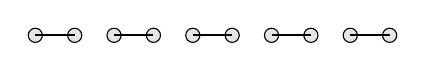
\begin{tikzpicture}[scale=0.5]
    \foreach \x in {0,1,2,3,4,5,6,7,8,9}
    {
      \draw[fill=gray!20] (\x,0) circle (0.18);
    }
    \draw[thick] (0,0)--(1,0);
    \draw[thick] (2,0)--(3,0);
    \draw[thick] (4,0)--(5,0);
    \draw[thick] (6,0)--(7,0);
    \draw[thick] (8,0)--(9,0);
\end{tikzpicture}
\caption{\small Majorana pairing pattern along the Kitaev chain in the trivial mode.}
\label{fig:kitaev-chain-trivial}
\end{figure}

The Topological Mode occurs when $|\Delta| = w > 0, \mu = 0$, where our Hamiltonian becomes:
\begin{equation}
    H = iw \sum c_{B,j}c_{A,j+1}
    \label{eq:kitaev_Hamiltonian_topological}
\end{equation}
Now the Majorana fermions pair with the adjacent spatial site, and we get unpaired fermions at $c_{A,1}$ and $c_{B,L}$

\begin{figure}[h]
\centering
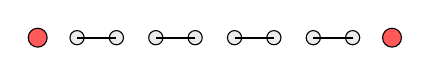
\begin{tikzpicture}[scale=0.5]
    \foreach \x in {0,1,2,3,4,5,6,7,8}{\draw[fill=gray!15] (\x,0) circle (0.18);}
      \draw[thick] (1,0)--(2,0);
      \draw[thick] (3,0)--(4,0);
      \draw[thick] (5,0)--(6,0);
      \draw[thick] (7,0)--(8,0);
      \draw[fill=red!65] (0,0) circle (0.24);
      \draw[fill=red!65] (9,0) circle (0.24);
      %\draw[dashed,thick,red!70] (0.2,0.35) .. controls (4.5,0.9) .. (8.8,0.35);
\end{tikzpicture}
\caption{\small Majorana pairing pattern along the Kitaev chain in the topological mode}
\label{fig:kitaev-chain-topological}
\end{figure}

% We can thus define a new fermionic operator from our Majorana fermions~\cite{Kitaev2000}:

% \begin{equation}
%     \tilde{a}_j=\frac{1}{2}(c_{B,j} + ic_{A,j+1}), \quad \tilde{a}_j^\dagger=\frac{1}{2}(c_{B,j} - ic_{A,j+1})
% \end{equation}

% Getting the new Hamiltonian:

% \begin{equation}
%     H = 2w\sum \left(\tilde{a_j}^\dagger\tilde{a_j} + \frac{1}{2}\right)
% \end{equation}

% The ground state gets annihilated by the operator $\tilde{a}_j$, but the states at the edges dont get annihlated, so acting with
% $c_{A,1}$ and $c_{B,2}$ on the ground state $|\psi_0\langle$ leaves it unchanged

However this is not restricted only to the case where $|\Delta| = w > 0, \mu = 0$, in the thermodynamical limit we find that
even for $\mu \neq 0$ there is still a topological phase given that $\Delta \neq 0$ and $|\mu| < 2w$~\cite{Herviou2017}, a deeper discussion of this will be held in section\ref{sec:Topology}.

To continue the analysis of our Hamiltonian it is advantageous to take our fermionic operators into momentum space, and work in the reciprocal space from now on:
\begin{equation}
    a_k = \frac{1}{\sqrt{L}}\sum a_j e^{ikj}, \quad a_k^\dagger = \frac{1}{\sqrt{L}}\sum a_j e^{-ikj}
    \label{eq:operators_momentum_space}
\end{equation}

With this our Hamiltonian in momentum space is:
\begin{equation}
    H_k = \sum (-\mu - 2w\cos(k))a_k^\dagger a_k +  i\Delta \sin(k)(a^\dagger_k a^\dagger_{-k} - a_{-k}a_k)
    \label{eq:Hamiltonian_momentum_space}
\end{equation}

We can also write our Hamiltonian as:
\begin{equation}
    H_k = \sum \Psi^\dagger_k h(k) \Psi_k
\end{equation}

Where $h(k)$ is a $2\times2$ Matrix and $\Psi_k$ is the Nambu vector:
\[
\Psi_k = \begin{pmatrix} a_k \\ a^\dagger_{-k} \end{pmatrix}
\]

So our matrix $h(k)$ is explicitly:
\[
h(k) = \begin{pmatrix}          \xi_k & 2i\Delta\sin(k)\\
                        -2i\Delta\sin(k)& -\xi_k \end{pmatrix}
\]

Where $\xi_k = -\mu - 2w\cos(k)$, the Hamiltonian's spectrum is:
\begin{equation}
    E_k = \sqrt{(\mu+2w\cos(k))^2+(2\Delta\sin(k))^2}
    \label{eq:energy_kitaev_chain}
\end{equation}

One is naturally interested in seeing how the energy differs between the two phases, and how the gap closes at the critical point, this is shown in figure~\ref{fig:bulk_dispersion} for different values of $\mu$ and $w$.
with some simple algebra we can see that at $k=0$ the energy reduces to $E_0 = |2w+\mu|$ and at $k=\pi$ we get $E_\pi = |2w-\mu|$, so the gap closes when $\mu = \pm 2w$.

\begin{figure}[ht]
    \centering
    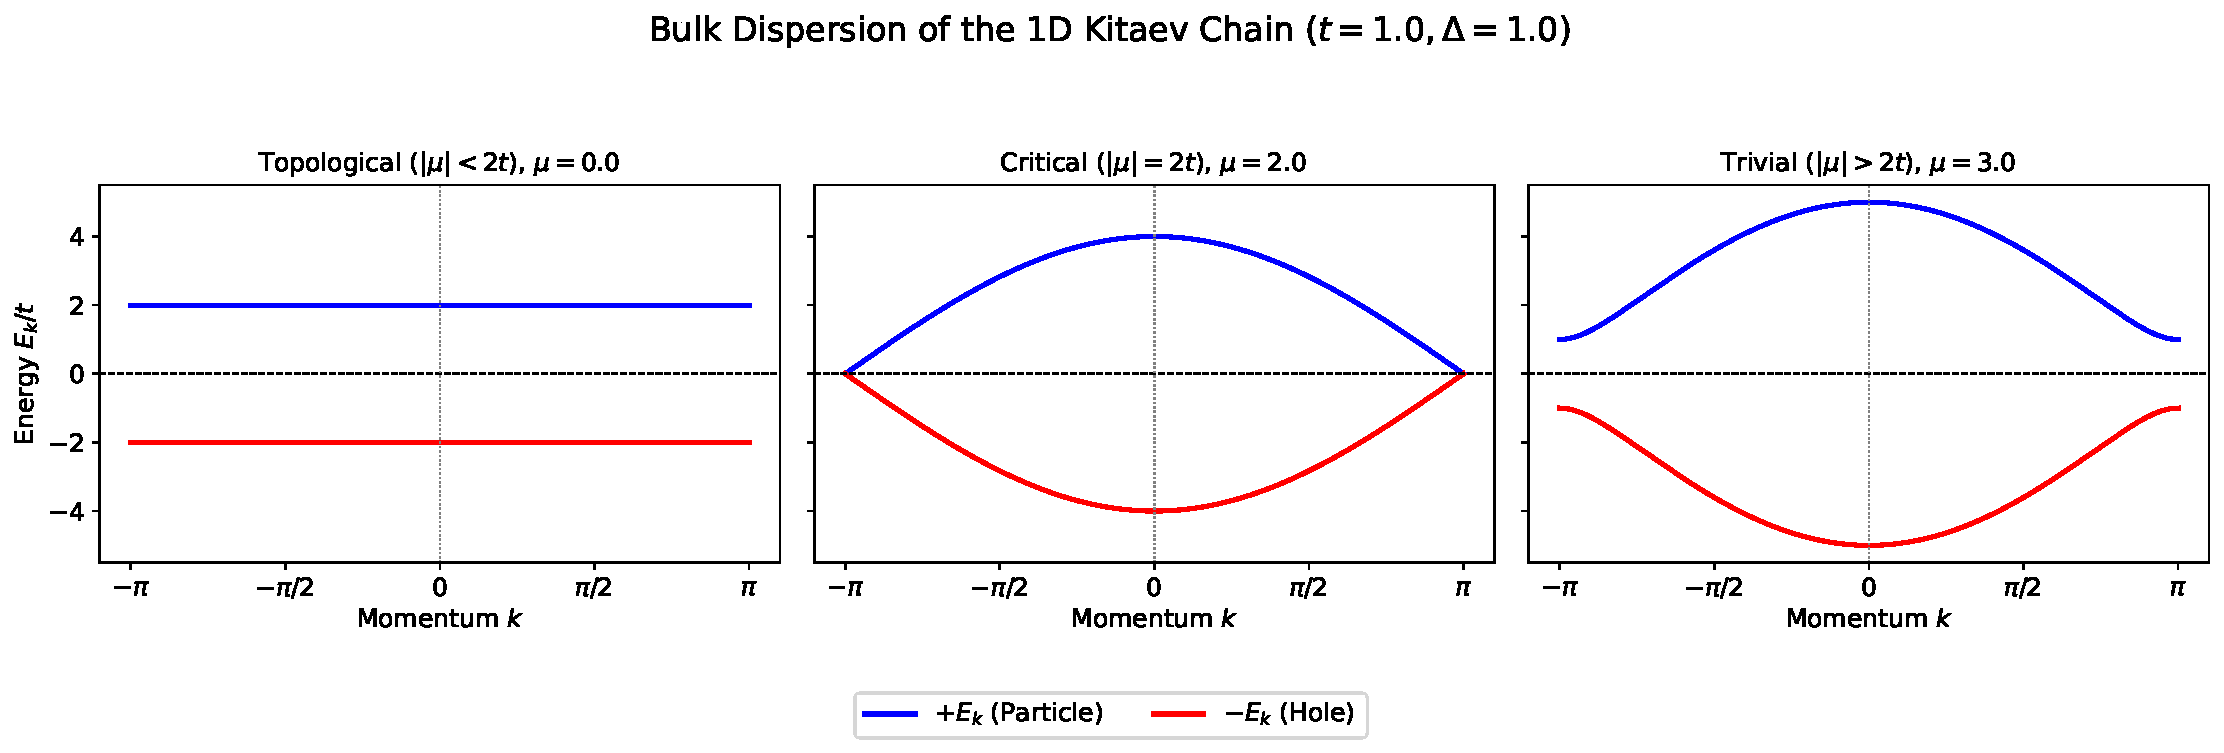
\includegraphics[width=0.8\linewidth]{../../../plots/block1_07_bulk_dispersion_panels.pdf}
    \caption{Bulk energy dispersion for different values of $\mu$ and $w$, ($t=w$).}
    \label{fig:bulk_dispersion}
\end{figure}

\newpage

This gives us an idea of when and where the phase transition between the trivial and topological modes occurs, but to further our understanding we first need a parameter that is 
solely dependent on the topology of the system, this is where the winding number comes into play. 

\section{Topology}\label{sec:Topology}

To construct the winding number first we rewrite the matrix $h(k)$ in terms
of the Pauli matrices:

\begin{equation}
    h(k) = -(\mu + 2w\cos(k)) \sigma_z - 2|\Delta|\sin(k)\sigma_y
\end{equation}

Now we can define the vector $\mathbf{n}(k) = -(2|\Delta|\sin(k), (\mu + 2w\cos(k)))$, this vector simplifies the visualisation of the 
topology of the Kitaev chain, we can see how $\mathbf{n}(k)$ behaves for different values of $\mu$ and $w$ in figure~\ref{fig:vector_n}:

\begin{figure}[ht]
    \centering
    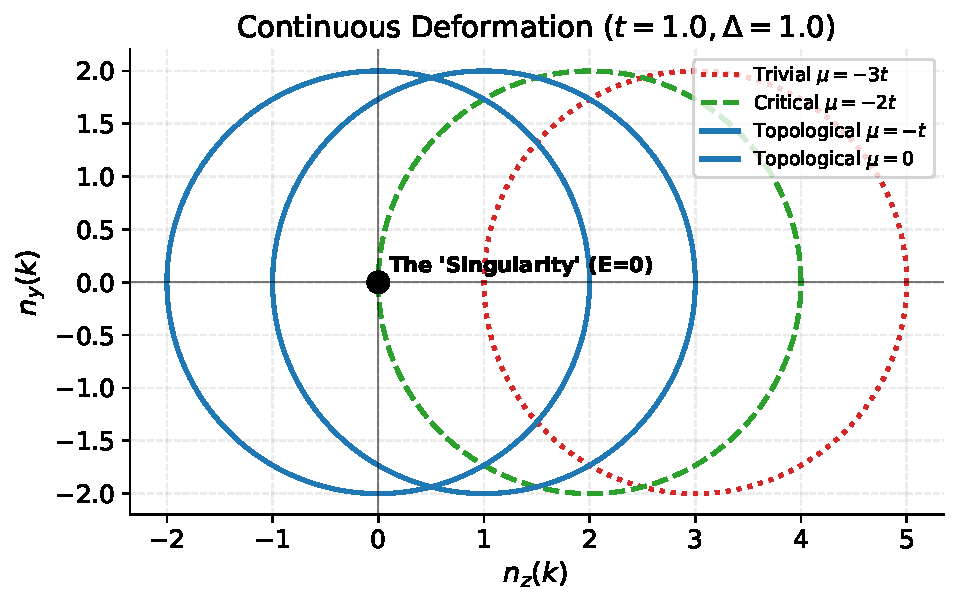
\includegraphics[width=0.5\linewidth]{../../../plots/block1_02_trajectory_deformation.pdf}
    \caption{$\mathbf{n}(k)$ for different values of $\mu$ and $w$, ($t=w$).}
    \label{fig:vector_n}
\end{figure}

The main difference between the trivial and topological case in the graph is the horizontal displacement, with the topological phase
encircling the origin, while the trivial phase stays outside that region, likewise the critical point occurs when the curve touches the origin.
Defining this property more rigorously we can define the winding number $\nu$ as follows:

\begin{equation}
    \nu =  \int \frac{d\theta_k}{dk}\frac{dk}{2\pi}
\end{equation}

Where $\theta_k$ is:
\begin{equation}
    \theta_k = \arg((\mu+2w\cos(k)) + i(2|\Delta|\sin(k)))
\end{equation}

This now gives us the full information of whether a specific configuration is trivial or topological for all possible $\mu,w,|\Delta|$, by telling us if the 
curve encompasses the origin or not.

\begin{figure}[ht]
    \centering
    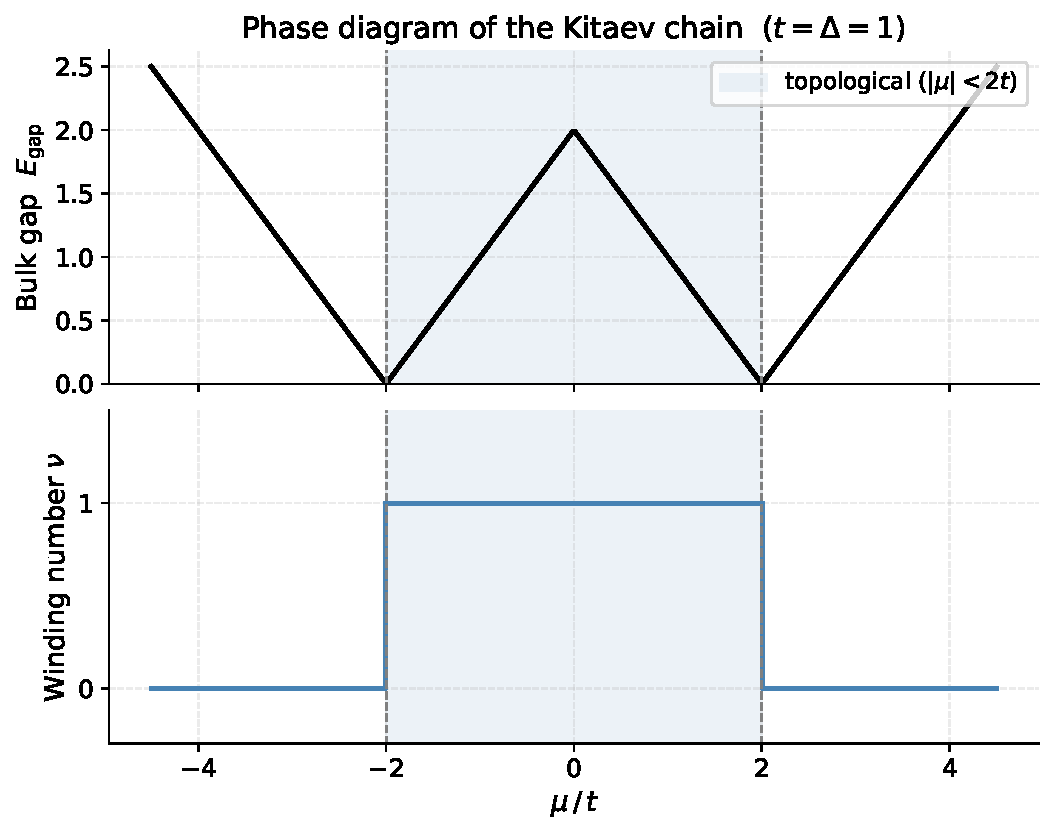
\includegraphics[width=0.5\linewidth]{../../../plots/block1_03_phase_diagram.pdf}
    \caption{$\nu$ for different values of $\mu$ and $w$, alongside the Bulk energy gap, ($t=w$).}
    \label{fig:phase_diagram}
\end{figure}

\section{Conclusion}

The Kitaev chain provides one of the simplest models for studying topological superconductivity and the emergence of Majorana edge modes. Depending on the values of the system parameters, the chain can exist in either a trivial or a topological phase. The transition between these phases occurs only when the bulk energy gap closes, highlighting the intimate connection between the bulk spectrum and the existence of edge states.

The topological properties of the system can be characterized by the winding number, a bulk topological invariant that distinguishes the two phases by describing the behavior of the Hamiltonian in momentum space. This provides a clear and intuitive framework for identifying the topology of the system without directly examining its edge states, illustrating the principle of bulk-boundary correspondence.

Although the Kitaev chain is an idealized model, it captures the essential physics of one-dimensional topological superconductors and serves as a fundamental example in the study of topological phases of matter. 
\subsection{Large Language Models as a Tool for Physics Research}

Throughout this course, one of our objectives was to evaluate and analyze how large language models (LLMs) can be integrated into physics research and the broader process of learning and scientific understanding.

In my experience, LLMs are a double-edged sword. On one hand, when used appropriately, they can significantly accelerate the learning process by gathering relevant resources, locating articles and reference material, and assisting with repetitive or time-consuming tasks. During this course, they proved particularly useful for compiling reports, preparing presentation slides, and supporting the implementation of code for the numerical simulations carried out in the later stages of the project.

On the other hand, excessive reliance on LLMs may lead to a false sense of understanding, as they can provide convincing explanations without encouraging the user to critically engage with the underlying concepts. They may also discourage the independent reasoning and analytical thinking that are essential when conducting scientific research. For this reason, I believe that LLMs should be regarded as tools that complement, rather than replace, traditional learning methods and critical thinking.

\subsection{Acknowledgments}

Throughout this report, the notation used for several variables differs from that adopted in the course slides, as I have predominantly followed the notation introduced by Kitaev in his original paper~\cite{Kitaev2000}. 
The use of large language models in the preparation of this report was limited to grammar correction, and assisting in locating relevant reference material.

\newpage
\printbibliography

\end{document}